\documentclass[11pt,a4paper,titlepage,oneside]{book}

\usepackage[czech]{babel}
\usepackage[utf8]{inputenc}
\usepackage{graphicx}
\usepackage{url}
\usepackage{fancyhdr}
\usepackage{setspace}
\usepackage{hyperref}
\usepackage{rotating}


%\usepackage{titlesec}
%\titleformat{\chapter}{\normalfont\LARGE\bfseries}{\thechapter}{1em}{}
%\titlespacing*{\chapter}{0pt}{3.5ex plus 1ex minus .2ex}{2.3ex plus .2ex}


\begin{document}

%nastavení fancy stylu
\lhead{
\includegraphics[height=0.5cm]{obrazky/lev.jpg} {ČVUT v~Praze}}
\rhead{\leftmark}
\cfoot{\thepage}
\setlength{\headheight}{24pt}

\pagestyle{empty}	%%vypne číslování

\begin{titlepage} %% titulní strana 1(bez lva)
	\begin{center}
		{\huge ČESKÉ VYSOKÉ UČENÍ TECHNICKÉ} \\ [0.25cm]
		{\LARGE FAKULTA STAVEBNÍ}
		\\[9cm]		
		{\Huge DIPLOMOVÁ PRÁCE}
		\\[9cm]
		{\Large Praha 2013 \hspace{\stretch{1}} Chrudoš VORLÍČEK}
	\end{center}
\end{titlepage}

\begin{titlepage} %%titulní strana 2 (se lvem)
	\begin{center}
		{\huge ČESKÉ VYSOKÉ UČENÍ TECHNICKÉ} \\
		{\LARGE FAKULTA STAVEBNÍ \\ [0.25cm]OBOR GEOINFORMATIKA}
		\\[1cm]
		\begin{figure}[!h]
		\begin{center}
		
\includegraphics[height=5cm]{obrazky/lev.jpg}
		\\[1cm]
		\end{center}
		\end{figure}							
		{\Huge DIPLOMOVÁ PRÁCE \\ [0.25cm]}
		{\LARGE \uppercase {Prototyp turistického systému zaloŽeného na datech \\[0.25cm] OpenStreetMap}}
		\\[3.5cm]
		{\Large Vedoucí práce: Ing. Martin LANDA, Ph.D. \\[0.25cm] Katedra geomatiky}
		\\[1cm]
		{\Large Praha 2013 \hspace{\stretch{1}} Chrudoš VORLÍČEK}
	\end{center}
\end{titlepage}

\newpage %%zadání
	\begin{center}
		\vspace*{15cm}
		{\Large ZDE VLOŽIT LIST ZADÁNÍ}
	\end{center}

%% Abstrakt
\begin{flushleft}
	\chapter*{}
	\section*{ABSTRAKT}
	\paragraph{} Hlavním tématem této práce je tvorba webové turistické aplikace za použití dat OpenStreetMap, jeho napojení na sociální síť Facebook a přidávání dat přímo do OpenStreetMap. Součástí práce je i stručné shrnutí existujích řešení, popsání užitých technologií a jejich výhod a nevýhod.
	\section*{KLÍČOVÁ SLOVA}
	{\sc{OpenStreetMap, OSM, Turistický systém, Facebook, Nette}}
	\section*{ABSTRACT}
	\paragraph{}
	\section*{KEYWORDS}
	{\sc{}}
\end{flushleft}

\newpage %%Prohlášení
	\vspace*{15cm}
	\section*{\Large PROHLÁŠENÍ}
		\paragraph{}Prohlašuji, že jsem diplomovou práci na téma \uv{Prototyp turistického systému založeného na datech OpenStreetMap} vypracoval samostatně a že veškerou použitou literaturu a podkladové materiály uvádím v~seznamu zdrojů.\\[1cm]
	V~Praze dne ....................... \hspace{\stretch{1}}................................. \\
	\hspace*{\stretch{1}} {(podpis autora)\hspace{0.25cm} }
	
\newpage %%Poděkování
	\vspace*{15cm}
	\section*{\Large PODĚKOVÁNÍ}
	\paragraph{}
		
\renewcommand{\baselinestretch}{1.5} %nastaví mezery
\newpage %%Obsah
\pagestyle{plain}
\pagenumbering{arabic}
\setcounter{page}{5}

	\tableofcontents

\newpage %%Obrázky a tabulky
	\listoffigures

\newpage %%Samotný text
%%Úvod
\chapter*{Úvod}
\addcontentsline{toc}{chapter}{Úvod}
	\paragraph{} Internet se stal součástí životů velkého množství lidí a s jeho rozšířením i do mobilních telefonů je dostupný na mnoha místech, kde bychom ho před lety nečekaly. Díky tomu lze využívat webové aplikace ikdyž jsme na cestách. Když jsme v horách či se jen touláme přírodou, mohou nám mapové portály pomoci s plánováním další cesty. Ve srovnání s globálními navigačními satelitními systémy(GNSS) mají tyto portály jen omezené možnosti lokalizace. Webové aplikace mohou na druhou stranu poskytnout doplňující informace o zajímavých věcech, kolem kterých nás mohou naše kroky zavést. Mapové portály se pro nás staly nepostradatelným pomocníkem při plánování cest či výletů. 
	\paragraph{} Stejně tak jako se liší služební cesta od výletu, liší se i potřeby uživatelů. Podnikatel cestující autem, který hledá nejkratší cestu z bodu A do bodu B, nepotřebuje pro vyhledávání turistické mapy. Ačkoliv je může použít, obsahují pro něj nadbytečná data a mohou být příliš podrobné. Kdyby turista hledal v automapě cestu z bodu A do B, pravděpodobně by ji našel, ale vedla by nejspíš po silnicích, což není úplně žádoucí. Každá mapa, ať už papírová či internetová, poskytuje různá data. Výhodou internetových mapových aplikací je mimo jiné i možnost zobrazení různých dat v potřebném měřítku v jednom mapovém okně.
	\paragraph{} Portály poskytující mapové aplikace často vytvářejí svá API, aby jejich produkty mohly být použity i na jiných serverech. Díky tomu je možné narazit na mapy od Googlu či Seznamu i na jiných stránkách. Jedná se o nejsnažší způsob, jak prezentovat prostorová data, např. společnost zabývající se venkovní reklamou tak může prezentovat rozmístění nabízených billboardů. Tento přístup má ale svá omezení daná funkcemi, které poskytuje API, a většinou i počtem přístupů či velikostí poskytovaných dat. Navíc se většinou jedná o doprovodnou funkci. Výhodou ovšem je snadnější tvorba. Pokud je zobrazování prostorových dat hlavní náplní aplikace, je lepší použít specializovanou aplikaci. Vytvoření takové aplikace vyžaduje mnohem více času a znalostí. 
	\paragraph{} Pro turistiku se dají použít oba zmíněné přístupy, ovšem jejich vhodnost závisí na zamýšlených funkcionalitách. Pro zobrazení možných cílů výletů lze využít API od některého z poskytovatelů. Z českých aplikací toto využívá Výletník.cz\ref{sec:vyletnik}. Pokud ale chceme prezentovat síť turistických stezek, vkládat vlastní trasy, editovat data atd., je lepší vytvořit vlastní systém, ve kterém budou požadované funkce dostupné.
	\paragraph{} Na internetu lze dohledat několik turistických portálů. Aby v rámci této práce nebylo vytvářeno něco, co už existuje, byl vytvořen vzorek aplikací. Tento výběr posloužil k utvoření přehledu funkcionalit, výhod, nevýhod a originálních prvků webových map. Více je pospáno v kapitole Existující řešení\ref{sec:Ex_reseni}. Většina nalezených aplikací neumožňuje připojení k sociálním sítím. V současné době, kdy jsou sítě jako Facebook a Twitter velmi rozšířené, mohou být funkce jako přihlášení přes už existující účet či sdílení výletních tras s přáteli přidanou hodnotou aplikace. 
	\paragraph{} Cíle této práce lze shrnout do několika hlavních bodů.
		\begin{itemize}
			\item Aplikace je postavena nad daty projektu OpenStreetMap.
			\item Pro přihlášení do aplikace lze použít účet na sociální síti Facebook. Pod tímto účtem pak lze zveřejňovat mapy na Facebooku.
			\item Přímo ze stránek projektu je možné editovat data projektu OpenStreetMap.
			\item Registrovaní uživatelé mohou přidat vlastní trasy. Jakýkoliv přihlášený uživatel může tyto trasy okomentovat.
			\item Registrovaní uživatelé mohou vkládat do mapy fotky.
		\end{itemize}
	\paragraph{} Protože v mapách často něco hledáme, měla by vyvíjená mapa umožnit uživatelům vyhledávat objekty a cesty z bodu A do bodu B. Vyhledávání by mělo zahrnovat i pokročilé volby, kdy se dá vyhledat zájmový bod v určité vzdálenosti od plánované cesty či od jiného bodu. Tyto body mají až druhotný význam a budou realizovány pouze v případě, že hlavní cíle projektu budou splněny.
	\paragraph{} Práce je strukturována do pěti kapitol. V první kapitole se text věnuje existujícím řešením. Prozkoumáním aplikací bylo zjištěno, jaké funkce jsou obvykle k dispozici a jaké nikoliv. Druhá kapitola je věnována  komunitnímu projektu OpenStreetMap. Bude zmíněna jeho historie, možnosti, kvalita a výhody a nevýhody. Protože aplikace používá data OpenStreetMap, budou v této kapitole popsána. Třetí kapitola je zaměřena na technologickou stránku problému. Množství programů a programovacích jazyků, které lze použít, je velké. Proto v této části budou popsány jen ty programy, jazyky a knihovny, které se použily či  jejichž použití bylo zvažováno. Ve čtvrté části práce je popsán vývoj a s ním spojené problémy. Též zde lze najít popsaný výsledný stav aplikace ke dni dokončení práce. V poslední, páté kapitole je zhodnocení celého projektu, odůvodnění koncového stavu a nápady na rozšíření, vylepšení či dodělání aplikace.
	
\pagestyle{fancy}

%%%%%%%%%%%%%%%%%%%%%%%
%%%%% EXISTUJÍCÍ ŘEŠENÍ 	   %%%%%
%%%%						      %%%%
%%%							  %%%
%%								     %%
%									 %
\chapter{Existující řešení}
	\label{sec:Ex_reseni}
	\paragraph{} Z velkého množství různých mapových aplikací bylo vybráno šest zástupců, kteří mají alespoň nějakou spojitost se zpracovávaným tématem. Kromě dvou v České republice nejčastěji užívaných mapových portálů GoogleMaps a Mapy.cz byly pro hodnocení zvoleny tři aplikace postavené nad daty OpenStreetMap. Jedná se o české aplikace OpenTrackMap a MTB mapa Evropy. Trojici uzavírá web Waymarked Trails. Poslední aplikací je už v úvodu zmiňovaný Výletník.cz, jehož mapová aplikace je vytvořena pomocí Google API. Každá z těchto aplikací je něčím specifická, má své výhody i nedostatky. 
	\section{Google Mapy}
		\url{http://www.google.com/maps/preview}
		\paragraph{} V globálním měřítku asi nejužívanější mapovou aplikací jsou Google Mapy spuštěné v roce 2005. Ve stejném roce společnost Google uvedla k mapám i API pro jejich použití na webech třetích stran. Podle typu užití se jedná buď o placenou či volně dostupnou službu. Google má k mapám velké množství doplňkových funkcí -- od vyhledávání míst přes vyhledávání cest autem, na kole či pěšky po Street View, zobrazení 3D modelů budov a fotek z momentálně zobrazené oblasti. Též lze importovata svá data a sdílet je s jinými uživateli.
		\paragraph{} Google Mapy sice jsou užitečným pomocníkem při plánování cest a zobrazení prostorových dat, ovšem jejich užití je pro turisty dosti omezené. Aplikace nedisponuje údaji o turistických stezkách. Důvodem, proč se mapy od Googlu dostaly do tohoto výběru, je aplikace Panoramio, která je na s mapami provázána. Jedná se vrstvu lokalizovaných fotografií, které uživatelé nahrály do aplikace. Možnost nahrát fotky do mapy sice poskytují i  Mapy.cz, ovšem aplikace Panoramio je starší -- vznikla v roce 2005. Původně nebyla vlastněna Googlem, ten ji získal v roce 2007 a v roce 2008 byla propojena s  mapovou aplikací. 
		\paragraph{}  Google vytvořil pro své mapy i nové zobrazení, které vychází z Mercatorova zobrazení. Pro zobrazení jsou použity vzorce pro Mercatorovo zobrazení na kouli, ale objekty mají  souřadnice v systému WGS 84, což vede k tomu, zobrazení není konformní.\label{google_mercator} Toto zobrazení má v označení EPSG:900913.

		\begin{figure}[!h]
			\begin{center}
				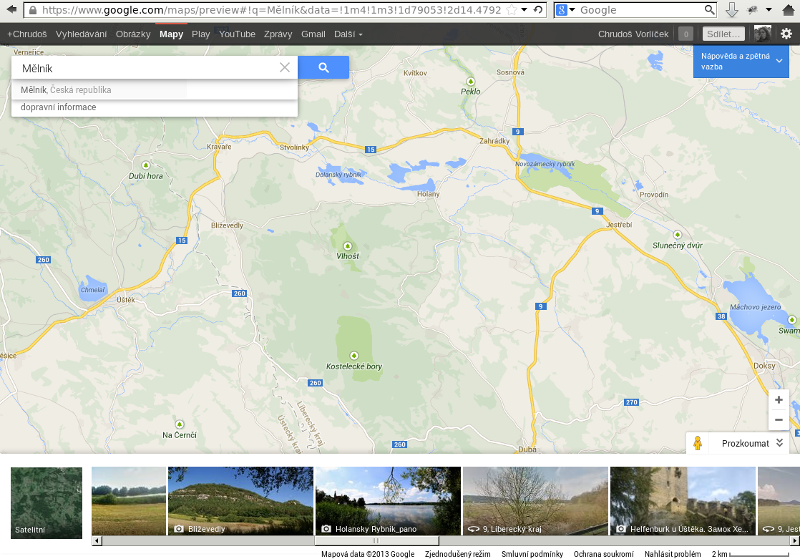
\includegraphics[width=12cm]{obrazky/googleMaps.png}
				\caption{Google Mapy s přehledem obrázků}
			\end{center}
		\end{figure}

			\begin{figure}[!h]
				\begin{center}
					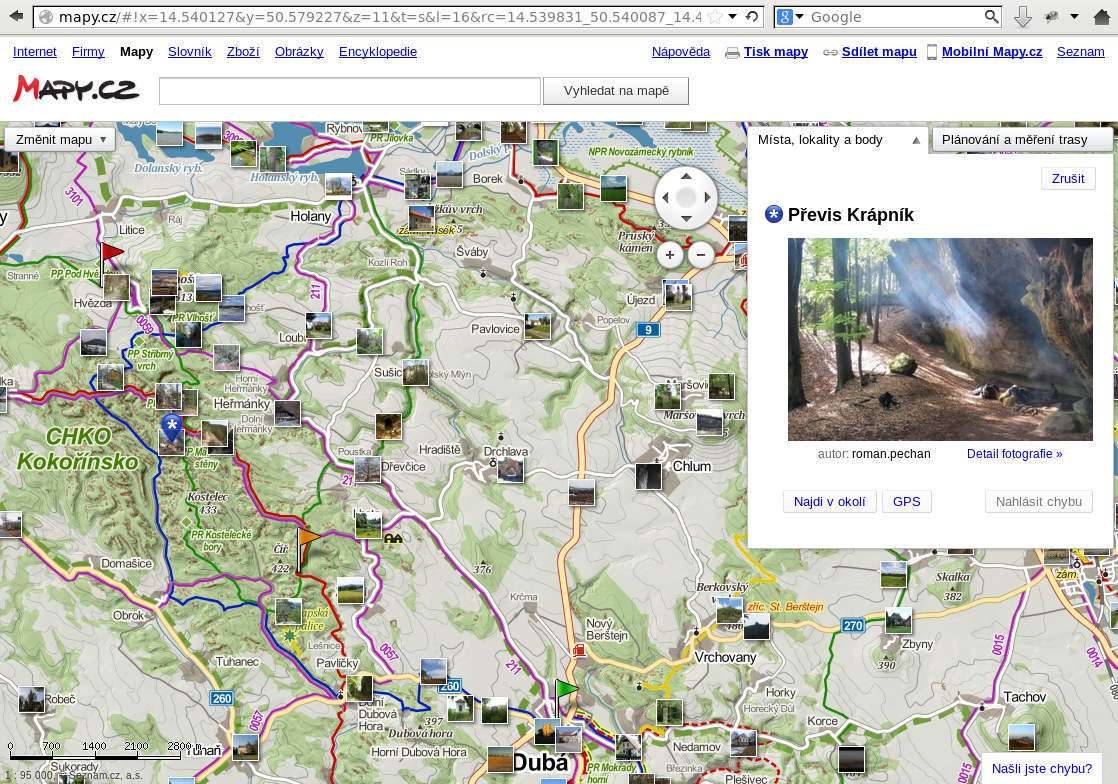
\includegraphics[width=12cm]{obrazky/mapycz.png}
					\caption{Turistická mapa na Mapy.cz}
				\end{center}
			\end{figure}

	\section{Mapy.cz}
		\url{http://mapy.cz/}
		\paragraph{} Ikdyž je Google se svými mapami světově nejužívanější, v českých podmínkách mu směle konkuruje mapová aplikace firmy Seznam. Mapy.cz mají oproti Googlu výhodu domácího prostředí a zaměření zejména na Českou republiku, což v důsledku znamená rychlejší aktualizaci mapových podkladů. Mapy.cz poskytují tři různé podkladové mapy (leteckou, obecnou a turistickou) a různé tématické vrstvy (turistické trasy, cyklotrasy, dopravní info, zastávky MHD a veřejné dopravy aj.). 
		\paragraph{} Na Mapách.cz mohou řidiči, cyklisti a chodci vyhledat trasy z bodu A do bodu B přes libovolný počet mezilehlých bodů. V závislosti na zvoleném dopravním prostředku bere vyhledávač v potaz i lesní cesty a turistické trasy. Ve stejné záložce lze najít i ruční měření vzdálenosti. Vyhledaná či ručně zadané cesta může být exportována. Též lze zobrazit její výškový profil. Do mapy lze přidat vlastní body a ty sdílet s ostatními uživateli pomocí url adresy. Stejně jako Google poskytuje i Seznam možnost vyhledávat místa podle souřadnic, ulice či názvu objektu. Mapy.cz podporují vkládání fotografií a jejich komentování, ale narozdíl od Googlu to není řešené jinou aplikací, ale je to přímo součástí aplikace.

		\begin{figure}[!h]
			\begin{center}
				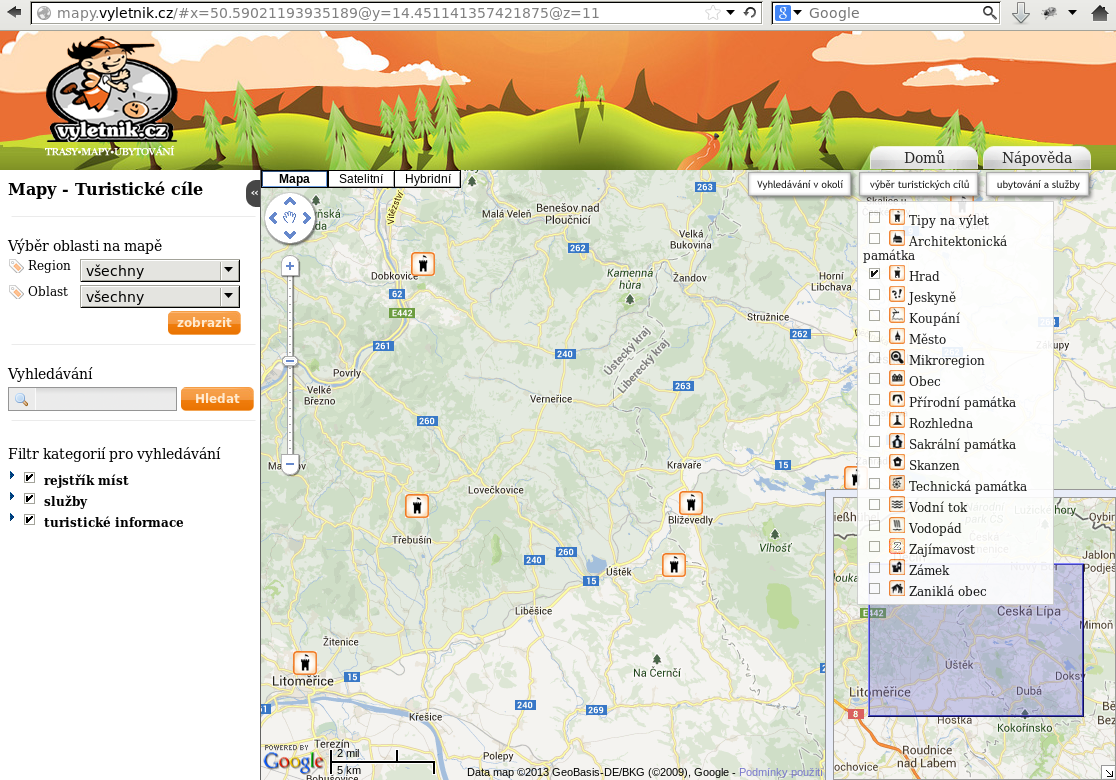
\includegraphics[width=12cm]{obrazky/vyletnik.png}
				\caption{Mapová aplikace portálu Výletník}
			\end{center}
		\end{figure}

	\section{Výletník}
		\label{sec:vyletnik}
		\url{http://mapy.vyletnik.cz/}
		\paragraph{} Turistický portál Výletník.cz poskytuje informace o možných cílech výletů, o službách spojených s turistikou (např. restaurace či ubytování)  či o zajímavých akcích. díky těmto datům je portál dobrým zdrojem nápadů, pokud připravujeme výlet. Registrovaným uživatelům poskytuje portál informace o akcích probíhajících následující víkend. Též uživatelům umožňuje vkládat vlastní fotografie, místa a příspěvky. Při registraci je inzerována možnost registrace pomocí Facebooku, ale nikde na to nebyl nalezen odkaz. Nakonec se ukázalo, že Adblock, doplněk prohlížeče Firefox blokující reklamy, vyhodnotil přihlašovací nástroj pro Facebook jako reklamu a podle toho s ním zacházel. Po vypnutí Adblocku propojení s Facebookem bylo viditelné. Na druhou stranu se objevilo množství reklam, které kazí jinak dobrý pocit z webu.
		\paragraph{} Pro mapovou aplikaci tohoto portálu platí to, co pro celý web -- všudypřítomné reklamy snižují přívětivost aplikace. Na několika místech se projevilo špatné nastylování aplikace, kdy se prvky překrývaly. Nejzřetelněji je to vidět na možnosti přepínání map. V nápovědě je napsáno, že aplikace poskytuje normální, satelitní a hybridní podkladovou mapu, ale možnost přepínání těchto map je překryta rozbalovacími seznamy zájmových bodů. Těch je k dispozici velké množství a jsou rozděleny na dvě základní skupiny -- \textit{turistické cíle} a \textit{ubytování a služby}. Obě skupiny obsahují další možnosti, ze kterých lze zvolit jednu či více položek. Výletník.cz umožňuje uživatelům vyhledávat objekty ve třech kategoriích:
			\begin{itemize}
				\item rejstřík míst,
				\item služby,
				\item turistické informace.
			\end{itemize}
Vyhledávat lze i v určitém okruhu od zvoleného bodu.
		\paragraph{} Ačkoliv tato aplikace poskytu solidní informace, má jistá omezení vyplívající z toho, že je vytvořena pomocí GoogleMaps API. Jednou z nevýhod jsou chybějící turistické a cykloturistické trasy. Google mapy tyto informace neposkytují a aplikace samotná je z jiných zdrojů nezískává, čímž vzniká nutnost pro užití dalších portálů pro plánování výletu.	
	
	\section{Waymarked Trails}
		\url{http://waymarkedtrails.org/cs/}
		\paragraph{} Aktuální přehled stezek pro turistiku, cykloturistiku a jízdy na inline bruslích je možno najít na mapě Waymarked Trails\cite{Waymarked}. Tato aplikace je vytvořena nad daty \textit{OpenStreetMap} a pokrývá celý svět. Největší množství dat je v Evropě, zbylé části světa jsou z velké části bez dat, ikdyž občas nějaká data obsahují. Nejvíce dat je poskytují vrstvy s turistickými a cykloturistickými stezkami. O poznání menší množství dat poskytují vrstvy pro horskou cyklistiku a inline bruslení.

		\begin{figure}[!h]
			\begin{center}
				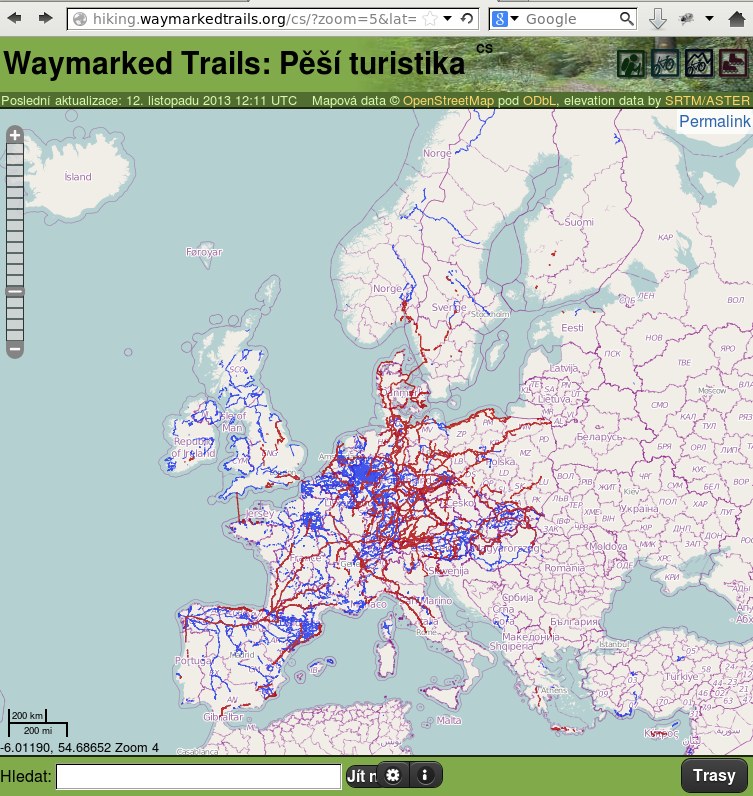
\includegraphics[width=8cm]{obrazky/waymarkedTrails.png}
				\caption{Hiking Map na Waymarked Trails}
			\end{center}
		\end{figure}
	
		\paragraph{} Velkou výhodou této mapy je poskytování informací o trasách a možnost jejich uložení v GPX formátu. Trasy jsou rozděleny na:
	\begin{itemize}
		 \item kontinentální -- mezinárodní trasy vedoucí přes několik států, značené prefixem E
		 \item národní -- trasy KČT
		 \item regionální -- trasy KČT
     		 \item ostatní -- naučné stezky, odbočky k hradům, zříceninám, vyhlídkám, přírodním zajímavostem apod.
	\end{itemize}
  Mapa také poskytuje možnost vyhledání místa podle názvu a vytvoření permanentního odkazu na mapový výřez. Mapa neposkytuje vyhledávání tras -- na to je potřeba použít jiná existující řešení, např. OpenRouteService (\url{http://www.openrouteservice.org/}), které kromě vyhledání trasy pro určitý typ dopravy (autem, na kole, pěšky) poskytuje i její export, výškový profil, vyhledání zájmových bodů v blízkosti.

 	\section{OpenTrackMap}
		\url{http://opentrackmap.cz/}
		\paragraph{} OpenTrackMap je projekt Ing. Radka Bartoně. Projekt běží na serveru geo102, který spravuje katedra Geomatiky na Fakultě stavební ČVUT v Praze. Tvorba této aplikace byla motivována snahou poskytnout mapy pro aplikaci TangoGPS běžící na platformě Openmoko\cite{OTM}. Již existující mapy nemohly být z licenčních důvodů či kvůli různým technickým omezením použity. Data OpenStreetMap mohou být volně použity, tudíž zde odpadá problém s licencí. Data jsou uložena v databázi PostgraSQL a pro jejich zobrazení je použit software Mapnik. Ačkoliv mapy v současné době nejsou aktualizovány, jejich přínos je ve vytvoření značkového klíče pro tras a objektů v mapě. 

		\begin{figure}[!h]
			\begin{center}
				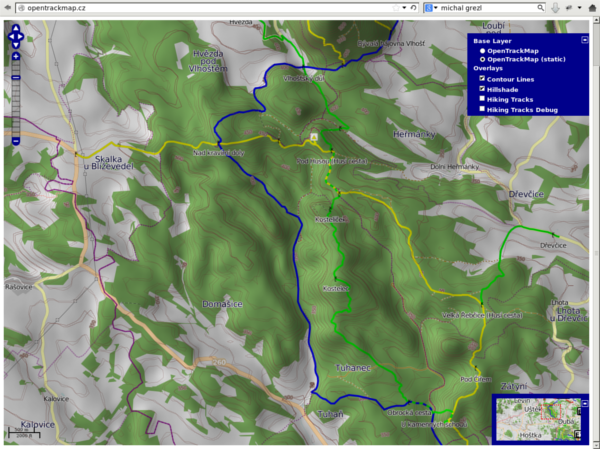
\includegraphics[width=12cm]{obrazky/otm.png}
				\caption{OpenTrackMap}
			\end{center}
		\end{figure}

		\paragraph{}  Aplikace poskytuje vrstevnice, stínování terénu, podkladovou mapu a turistické trasy. Vzhledem k tomu, že mapy byly určeny pro zobrazení v mobilních zařízeních, bylo zapotřebí snížit množství dat přenášených k uživateli. Toho bylo dosaženo pomocí dlaždic. Původní testování odhalilo, že pro malá měřítka je vykreslování pomalejší, protože je pro velkou oblast vykreslováno stínování kopců. Od určitého stupně přiblížení se rychlost vykreslení mírně zvýšila, protože byla vykreslována menší plocha a protože klesl počet vektorových prvků.

	\section{MTB mapa Evropy}
		\url{http://mtbmap.cz/}
		\paragraph{} Projekt Martina Tesaře MTB mapa Evropy byl původně bakalářskou prací zpracovávanou na fakultě informatiky Masarykovy univerzity v Brně. Aplikace prezentuje stezky pro jízdu na horském kole. Mapa byla původně omezena pouze na oblast České republiky a přilehlého okolí, ale časem byla rozšířena na Evropy. Mapa využívá značkový klíč projektu OpenTrackMap, který je popsán na OpenStreetMap Wiki\cite{otm_klic}, a kromě cyklistických stezek zobrazuje i turistické cesty. Aktuálnost mapy je udržována týdenními aktualizacemi dat OpenStreetMap. Data pochází ze serveru \textit{geofabrik.de}, který poskytuje možnost stažení dat OpenStreetMap pro jednotlivé země, kontinenty i celý svět.
		\paragraph{} Apliakce poskytuje velké množství funkcí, které jsou dostupné všem. K dispozici je vyhledávání pomocí služby OpenStreetMap Nominatim\cite{nominatim}. Dále lze exportovat data v souřadnicemi daném výřezu. Zde lze nastavit stupeň přiblížení, velikost výsledku v pixelech a zobrazené mapové prvky -- tiráž. název mapy, trasu, legendu a měřítko. Kromě vyhledávání míst  pomocí Nominatim je k dispozici i vyhledání cesty podle množství vstupních parametrů, které zahrnují například typ cesty, druh povrchu nebo obtížnost. Tyto parametry jde uložit na disk a později je znovu použít pro vyhledání stejné cesty. Lze též vložit vlastní cestu v souboru GPX nebo ručně a zobrazit k ní výškový profil. Taktop vytvořené stezky se zobrazí v mapě, ale neukládají se pro pozdější zobrazení. Aplikace umožňuje vygenerovat permanentní odkaz na zobrazenou pozici či přesměruje uživatele na OpenStreetMap a otevře editor iD.
		\paragraph{} Tento projekt má svoji stránku i na OpenStreetMap Wiki, kde jsou popsány úkoly, kterými by měl směřovat další vývoj aplikace. Mapa byla původně vytvořena v OpenLayers\cite{tesar_bp}, ale v současné době užívá javascriptovou knihovnu Leaflet. K dispozici jsou 4 podkladové mapy (MTB mapa, OSM Mapnik, OpenCycleMap, Hike \& Bike Map), které jsou zobrazeny v EPSG:3857. Toto zobrazení je ekvivalentní s EPSG:900913, které na svých mapách používá Google. Jak bylo uvedeno výše\ref{google_mercator}, toto zobrazení není přesně konformní, ovšem v tiráži je uvedeno \uv{Zobrazení: Konformní válcové - mercatorovo}.
		\begin{figure}[!h]
			\begin{center}
				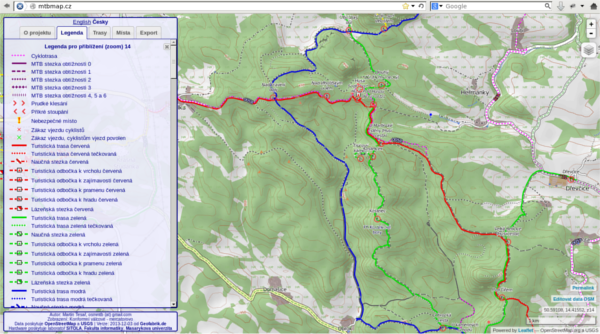
\includegraphics[width=12cm]{obrazky/mtb.png}
				\caption{MTB mapa Evropy}
			\end{center}
		\end{figure}

%%%%%%%%%%%%%%%%%%%%%%%
%%%%% OPEN STREET MAP        %%%%%
%%%%						      %%%%
%%%							  %%%
%%								     %%
%									 %
\chapter{OpenStreetMap}
	\section{O Projektu}
		\paragraph{} Tato práce je navázána na projekt OpenStreetMap a toto jméno se zde velice často objevuje. Z toho důvodu by bylo vhodné říci o co se jedná, jakou má projekt historii, jak v současné době vypadá a jaké má využití. 
		\paragraph{} OpenStreetMap je svobodná mapa, kterou vytváří a spravují její uživatelé. Narozdíl od jiných mapových děl OpenStreetMap poskytují uživatelům možnost stáhnout si data a volně s nimi nakládat. Díky možnosti svobodného nakládání s daty vznikají různá mapová díla dle potřeb uživatelů. Mapa musí mít uvedeno autorství OpenStreetMap contributors a musí být šířena pod stejnou licencí jako samotná OpenStreetMap. Toto je známo jako licence \textit{CC BY-SA 2.0}\cite{creative_commons}.
		\paragraph{}Projekt vznikl ve Velké Británii v roce 2004. O jeho základy se postaral Steve Coast, který se nechal inspirovat jiným komunitou řízeným projektem -- svobodnou encyklopedií Wikipedie. O dva roky později vznikla OpenStreetMap Foundation, která projekt podporuje. V průběhu let povolily některé společnosti používat své mapové podklady pro tvorbu OpenStreetMap. V roce 2006 to byl Yahoo. O rok později Automotive Navigation Data poskytla mapy silniční sítě Nizozemska, Indie a Činy. 
		\paragraph{} Od vzniku aplikace vzrostl počet registrovaných uživatelů až na milion. V srpnu 2008 měla aplikace 50 000 registrovaných uživatelů. Do konce následujícího roku narostlo toto číslo na skoro na  200 000. V roce 2012 služba registrovala 600 000 členů a 6. ledna 2013 překročil počet uživatelů 1 milion. Ze statistik vyplývá, že kolem 30\% uživatelů vytvořilo alespoň jednu sadu změn\cite{neis}. 
		\begin{figure}[!h]
			\begin{center}
				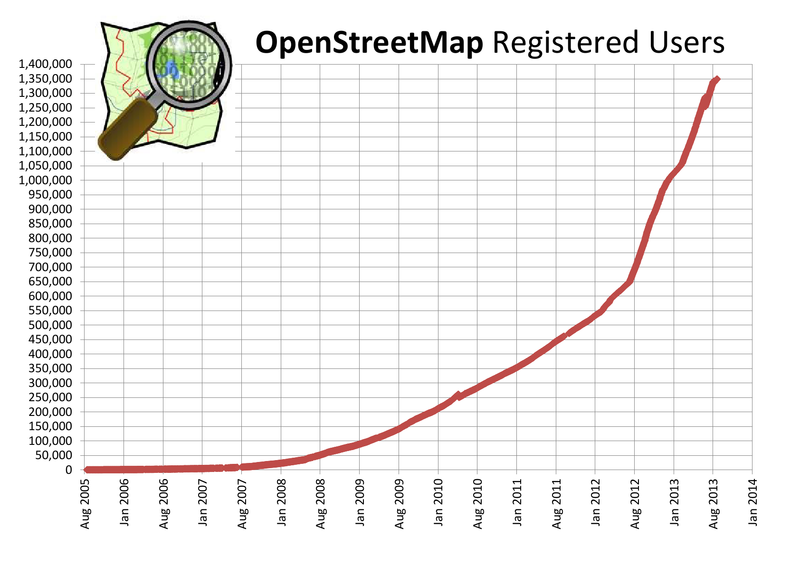
\includegraphics[width=12cm]{obrazky/osm_stat_users.png}
				\caption{Graf nárustu registrovaných uživatelů}
			\end{center}
		\end{figure}

	\section{Data}
		\subsection{Typy dat}
		\paragraph{} Jak už bylo řečeno, data pořizují samotní uživatelé mapy, což má za následek velké množství rozličných dat. Kromě standartních objektů, jako jsou silnice, vodstvo, budovy, zalejsněné oblasti či turistické značky, jsou mapovány i věci, které na normálních mapách zobrazeny nejsou. Jedná se například o bezpečnostní kamery na veřejných místech. Data mohou být:
	\begin{itemize}
		\item uzly (nodes) -- body se souřadnicemi,
		\item cesty (ways) -- liniové prvky a hranice polygonů -- nebo
		\item relace (relations) -- popisují vztahy s dalšími prvky.
	\end{itemize}
Kromě těchto tří elementů mohou mít prvky své tagy, do kterých se zaznamenávají  vlastnosti. 			\paragraph{}Uzly mají přiřazeny zeměpisné souřadnice a identifikátor (id). Volitelně může být prvku přiřazena i výška. Uzly mohou být samostatné prvky (např. rozcestník či sloup) nebo jsou součástí cesty. V tom případě definují tvar cesty. Uzly musí být na spojnicích více cest -- např. když se protínají dvě cesty, tak součástí obou cest musí být stejný vrchol. Pokud by to tak nebylo, nejednalo by se z topologického hlediska o křižovatku, ale mimoúrovňové křížení. Globální dataset obsahuje k roku 2013 přes 2 x 10$^9$ uzlů.

		\begin{figure}[!h]
			\begin{center}
				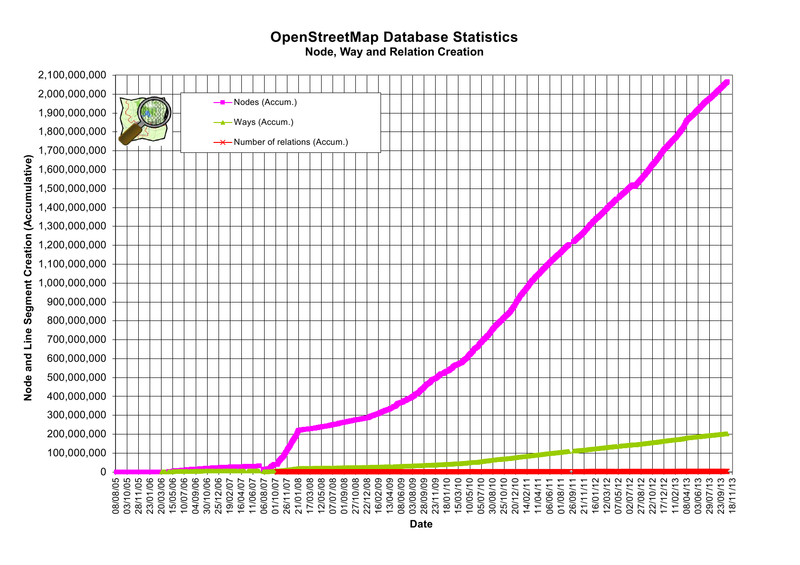
\includegraphics[width=12cm]{obrazky/osm_stat_elements.png}
				\caption{Graf vývoje počtu uzlů, cest a relací}
			\end{center}
		\end{figure}

		\paragraph{} Oproti uzlům je cest výrazně míň (kolem 200 000), protože cesty jsou tvořeny 2 až 2000 uzly spojenými liniovými segmenty. Cesta je buď otevřená nebo uzavřená. Otevřená cesta je taková, kde začátek a konec tvoří jiný uzel. Uzavřená cesta má identický počáteční a koncový uzel. V tomto případě se může jednat o uzavřenou polylinii či plošný prvek. Rozdíl lze stanovit pomocí tagu area -- pokud má hodnotu yes, jedná se o plochu. V některých případech může cesta tvořit polylinii a hranici polygonu zároveň -- toto je pak označeno odpovídajícím způsobem ve vlastnostech.

		\begin{figure}[!h]
			\begin{center}
				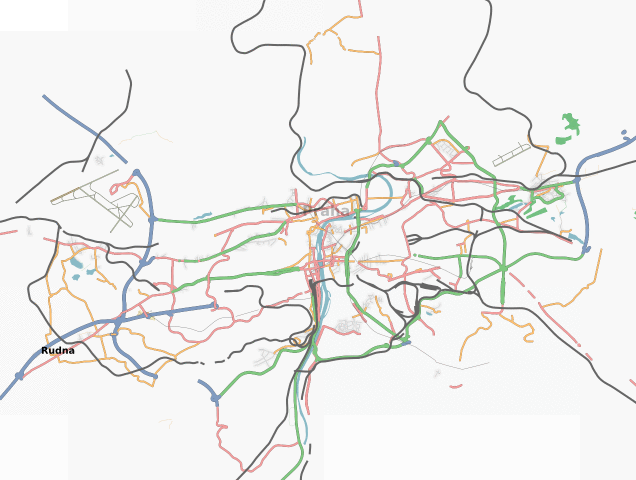
\includegraphics[width=12cm]{obrazky/Osm-200607-praha.png}
				\caption{Praha na mapách OpenStreetMap -- červenec 2006}
				\label{fig:praha2006}
			\end{center}
		\end{figure}

		\paragraph{} Vznik dat se dá rozdělit do tří skupin. První z nich je přímý sběr v terénu, kdy uživatel chodí venku a pomocí GPS přístroje získává souřadnice, které pak importuje v souboru GPX do mapy. Druhou variantou je odvozování z existujících mapových děl. Zde je ovšem potřeba dávat pozor, aby podklady pro odvození  byly kompatibilní s licencí, kterou užívá OpenStreetMap. V případě, že nejsou vyjasněny licenční podmínky,materiály použity být nemohou. Pro odvozování na území České republiky se dá kupříkladu použít ortofoto poskytované přes WMS Ústavem pro hospodářskou úpravu lesů (ÚHÚL) či WMS katastrální mapy Českého úřadu zeměměřického a katastrálního(ČÚZK). WMS ortofotomapy ČÚZK na odvozování nemůže být použita. Může být ale použita na ověření přesnosti jiných použitelných zdrojů.

		\begin{figure}[!h]
			\begin{center}
				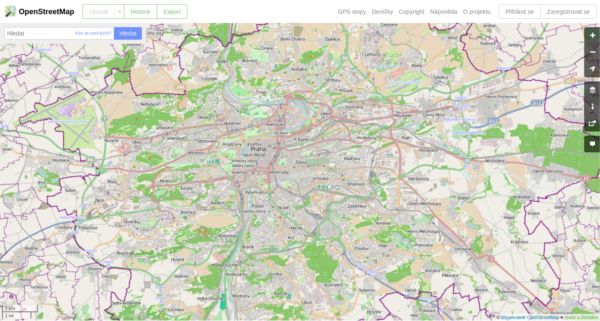
\includegraphics[width=12cm]{obrazky/Osm-201312-praha.png}
				\caption{Praha na mapách OpenStreetMap -- prosinec 2013}
				\label{fig:praha2013}
			\end{center}
		\end{figure}

		\paragraph{} Graf vývoje počtu elementů ukazuje, že z počátku přibývalo malé množství objektů a větší zvrat nastal spolu s nárustem počtu uživatelů. V roce 2007 je vidět skokový nárust počtu bodových prvků -- jedná se o data silniční sítě Nizozemska, Indie a Číny poskytnuté organizací Automotive Navigation Data. 
		Přibývání počtu prvků v mapě lze též dobře sledovat na malých plochách. Pro ilustraci jsou zde přiloženy obrázky, jak Praha byla zmapována v roce 2006 \ref{fig:praha2006} a v prosinci 2013 \ref{fig:praha2013}. V prvním případě jsou zmapovány hlavní silnice a vodní toky, zatímco druhý obrázek je plnohodnotnou mapou.
	
	\subsection{Uložení dat}
		\paragraph{} Data se ukládají do databáze, která je klíčovým prvkem celého projektu. Pro každý typ prvku existují tabulky v databázi. Kromě současné verze obsahuje databáze i historické verze, takže lze dohledat změny a případně je vrátit. Další tabulky se vztahují ke změnovým sadám (changesetům), GPX souborům nebo registrovaným uživatelům. Kromě tabulek jsou uloženy i primární a cizí klíče, sekvence a indexy.
		\paragraph{} Data jsou distribuovány v XML souboru Planet.osm, který je vytvářen v týdenních intervalech. V současnosti je velikost nekomprimované sady přes 400 GB, při užití komprimace je možno se dostat k 29 GB. Protože dost často není potřeba mít data z celého světa, dělají se i extrakty, které pokrývají jednotlivé kontinenty, země nebo města. Tyto výtahy jsou vytvářeny častěji -- \url{http://download.geofabrik.de} poskytuje data s denním intervalem. Vytvoření obrazu databáze většinou zabere 12 hodin\cite{planet.osm}.
	\paragraph{} Kromě samotných mapových dat jsou k dispozici i planet.gpx s údaji z nahraných GPX souborů a soubor s historií, který obsahuje každou revizi každého objektu. Planet.gpx obsahuje v nekomprimovaném stavu 55 GB dat, historie změn kolem 500 GB. 
	\paragraph{} Data jsou uložena na databázovém serveru, který má dostatečné prostředky pro správu těchto dat. Od dubna 2009 do dubna 2012 byl primárním serverem server Smaug. Operační systém Ubuntu 12.04 LTS Server amd64 obsluhuje relační databázi PostgreSQL ve verzi 9.1. Pevné disky mají kapacitu přes 6 TB a operační paměť je 64 GB. V současné době je primírním serverem server se jménem Ramoth, který je také obsluhován operačním systémem Ubuntu 12.04 LTS Server amd64, ovšem od svého kolegy se liší jak kapacitou disků (skoro 15 TB), tak operační pamětí (256 GB). Funkci databázového systému plní stále PostgreSQL 9.1.
	\paragraph{}Každý záznam v databázi má u sebe uvedeny i své vlastnosti. Protože pro každý typ prvku je jedna tabulka, jsou některé vlastnosti prvku prázdné. Parametry, které se evidují např. u silnice jsou jiné než vlastnosti, které nás zajímají u řeky -- obojí lze najít v tabulce s liniovými prvky. Aby se běžný uživatel či vývojář vyznali v databázi, jsou vytvořeny na wiki projektu stránky, které popisují všechny parametry (sloupce v databázi) a hodnoty, kterých můžou nabývat. Díky tomu je hlednání v databázi vůbec možné a nepřipomíná hledání v jehly v kupce sena.


	\section{Editory} % id, Potlach 2, JOSM, Merkaator
		\paragraph{} Součástí práce je napojení editoru vytvářené aplikace na data OpenStreetMap. Stojí tedy za zmínku, jaké jsou prostředky, kterými se v současné době provádí editace dat. 
		\subsection{iD}
			\paragraph{}Editor iD je nejnovějším z uvedených editorů. Pro užití na OpenStreetMap byl spuštěn v květnu 2013. Jedná se o javascriptovou aplikaci, která je šířena pod licencí WTFPL (Do What the Fuck You Want to Public License)\cite{wiki_wtfpl}, která umožňuje naprosto volně nakládat s produktem. K vykreslení je užívána javascriptová knihovna d3js, která slouží k práci v na datech založených dokumentech. Knihovna užívá HTML, CSS a SVG k vykreslení požadovaných prvků. Podpora jiných vykreslovacích přístupů není zatím v editoru iD implementována. Jedná se o aplikaci vhodnou pro začátečníky, protože má jednoduché ovládání.

		\begin{figure}[!h]
			\begin{center}
				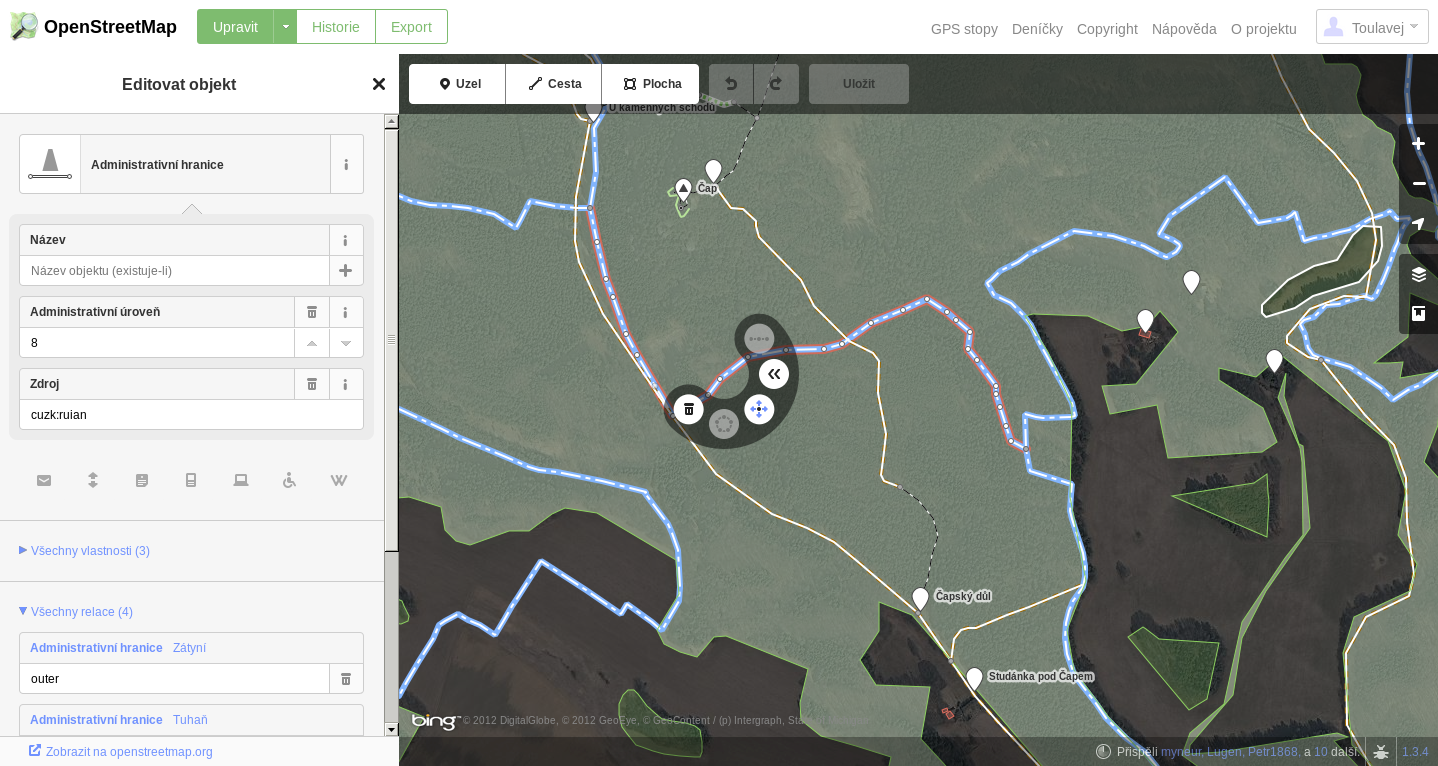
\includegraphics[width=12cm]{obrazky/iD_osm.png}
				\caption{Editor iD na webu OpenStreetMap.org}
				\label{fig:iD_osm}
			\end{center}
		\end{figure}

			\paragraph{} Podle stránek projektu\cite{wiki_iD} program zatím plně nepodporuje prohlížeče Internet Explorer verze 9, 10 a 11. Někteří uživatelé též hlásili zhoršený výkon pro prohlížeč Firefox.

		\subsection{JOSM}
			\paragraph{}JOSM (Java OpenStreetMap Editor) je na javě založený editor dat OpenStreetMap. Jedná se o desktopovou aplikaci s licencí GPL (General public license), ze které jsou změny dálkové nahrávány do hlavní databáze. Narozdíl od iD poskytuje JOSM mnohem více možnostní pro manipulaci s daty, což je znát i na jeho uživatelském rozhraní\ref{fig:josm_osm}. Aplikace podporuje čtení GPX souborů buď z pevného disku nebo z databáze OpenStreetMap, editování existujících uzlů, cest, tagů a relací.
		\begin{figure}[!h]
			\begin{center}
				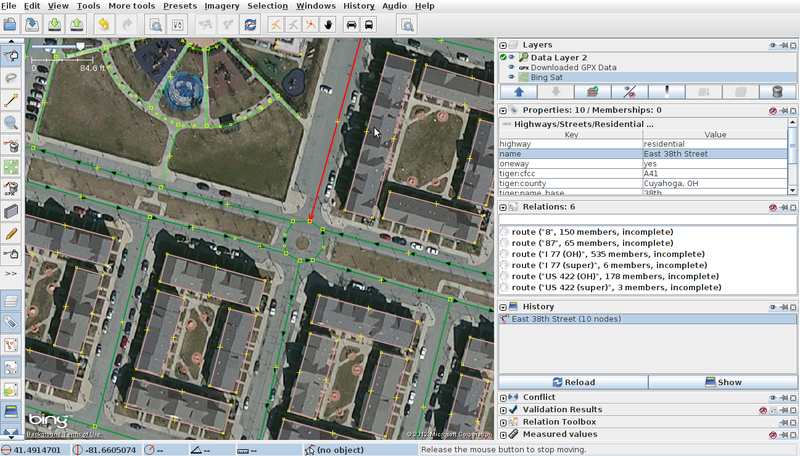
\includegraphics[width=12cm]{obrazky/josm_osm.png}
				\caption{Editor JOSM (zdroj: OSM Wiki\cite{wiki_josm})}
				\label{fig:josm_osm}
			\end{center}
		\end{figure}
			\paragraph{} Výhodou oproti online editorům je možnost pracovat i bez připojení k internetu. Aplikace také poskytuje různá rozšíření, která z ní dělají velmi silný editovací nástroj. Dle informací na OpenStreetMap Wiki\cite{wiki_josm} je práce s tímto editorem jednoduchá. Některé pokročilejší funkce mohou mít složitější ovládání a jejich zvládnutí může zabrat čas.

		\subsection{Merkaator}
			\paragraph{} Editor Merkaator je určen pro Unix, Mac OS i Windows a je distribuován pod licencí GNU GPL v2. Editor je ve stádiu vývoje (dle OpenStreetMap Wiki je dostupná verze 0.18.1 vydaná v červnu 2012), ovšem vývojářská komunita tohoto projektu není příliš aktivní. Aplikace obsahuje prvky, které stojí za povšimnutí. Jedná se například o průhledné zobrazení vrstev, editor stylů zobrazení mapy, přímé připojení k GPS přijímači nebo vykreslení mapy do SVG nebo bitmapového obrázku za použití momentálně užitých stylů. Vzhledem k tomu, že je program ve vývoji, lze některé prvky získat pouze kompilací ze zdrojových souborů, což pro většinu uživatelů není vhodné.

		\begin{figure}[!h]
			\begin{center}
				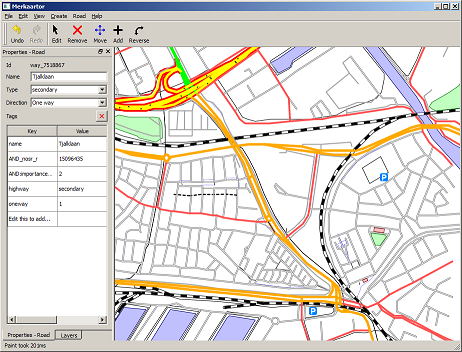
\includegraphics[width=12cm]{obrazky/merkaator_osm.png}
				\caption{Editor Merkaator (zdroj: OSM Wiki\cite{wiki_merkaator})}
			\end{center}
		\end{figure}

		\subsection{Potlatch 2}
			\paragraph{} Stejně jako iD editor je i Potlatch 2 online editor s licencí WTFPL, ale narozdíl od něj je napsán ve Flashi. Jedná se o jednoduchý editor, který není určen pro náročnější uživatele. Potlatch 2 vznikl kompletním přepsáním původního Potlatch, kdy byly přidáno zobrazení WYSIWYG (What You See Is What You Get), jednodušší tagování a autentizace přes OAuth pro zakomponování do jiných stránek při zachování napojení na OpenStreetMap. Z důvodu existence editoru iD není v současnosti aplikace aktivně vyvíjena.

		\begin{figure}[!h]
			\begin{center}
				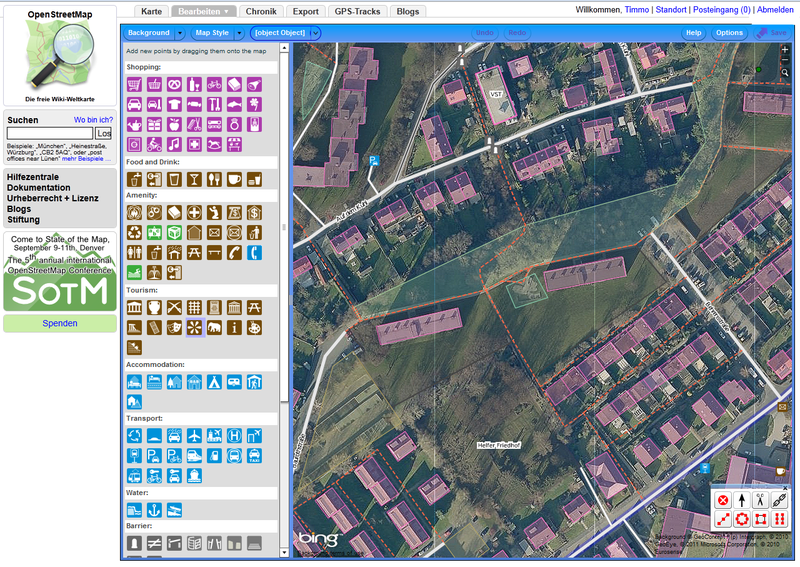
\includegraphics[width=12cm]{obrazky/p2_osm.png}
				\caption{Editor Potlatch 2 (zdroj: OSM Wiki\cite{wiki_p2})}
			\end{center}
		\end{figure}

	\section{Využití}  %napojení na další stránky
		\paragraph{} Data OpenStreetMap jsou široce využívány k tvorbě tématických map, např. z oblasti turistiky. Mapy mohou též sloužit jako podklady do navigací. Ačkoliv tyto produkty ocení většina uživatelů, dle mého leží větší význam map OpenStreetMap v oblasti humanitární pomoci.
		\paragraph{}V momentě, kdy nějakou část světa zasáhne živelná katastrofa, mohou dobrovolníci z řad uživatelů OpenStreetMap z aktuálních družicových snímků vytvořit novou aktuální mapu postižené oblasti. Toto bylo využito třeba v roce 2010, kdy bylo Haiti zasaženo zemětřesením, a v současnosti probíhá nové mapování po tajfunu na Filipínách z listopadu 2013. Během prvního týdne od tajfunu bylo editováno víc jak 2 000 000 objektů a do obnovy se zapojilo přes 900 uživatelů. K 11.prosinci 2013 bylo za přispění více jak 1 600 uživatelů zmapováno přes 4,5 milionu objektů\cite{wiki_tajfun}.
		\paragraph{} Aby bylo zajištěno efektivní tvorba, produkce a distribuce map pro postižené oblasti, byla v lednu 2009 vytvořena skupina Humanitarian OpenStreetMap Team\cite{wiki_hot}, která tuto činnost řídí.
	

%%%%%%%%%%%%%%%%%%%%%%%
%%%%% POUŽITÉ TECHNOLOGIE%%%%%
%%%%						      %%%%
%%%							  %%%
%%								     %%
%									 %
\chapter{Použité technologie}
	\paragraph{} Pro potřeby této práce byly užité technologie rozděleny na servery, které zpracovávají data, databázi a její doplňky a užité programovací jazyky. V této kapitole budou všechny postupně popsány.
%%%Servery
	\section{Servery}
		\paragraph{} Serverem rozumíme aplikaci běžící na počítači, která zpracovává dotazy a posílá odpovědi. Podle toho, jaké požadavky daný server zpracovává, mluvíme o webovém (web server), poštotovním (mail server), databázovém (database server), mapovém (map server) a jichých serverech. Protože se jedná o programy, tak je možné, aby na jednom stroji běželo velde sebe i více serverů. Pro potřeby této datové aplikace byl využit webový server Apache HTTP Server\cite{apache} a mapový server Geoserver.
		\subsection{Apache HTTP Server}
			\paragraph{} Jak už bylo řečeno v předchozím odstavci, Apache HTTP Server (častěji označován pouze jako Apache) je webový server. Jeho funkce spočívá v přijímání požadavků, jejich zpracování a odeslání odpovědi. Zpracováním se rozumí např. odeslání statické webové stránky nebo předání požadavku dalším aplikacím. Samotná komunikace je zajištěna přes hypertextový přenosový protokol (HTTP -- HyperText Transfer Protokol) Množství možných modulů značně rozšiřují možnosti samotného jádra programu. Příkladem modulu může být mod\_rewrite, který slouží k přepisování URL adresy, mod\_php rozšiřující Apache o podporu PHP nebo mod\_ssl pro šifrované spojení. Tento výčet je jen malou částí množiny.
			\paragraph{} Apache je open--source free--to--use software, což znamená, že kdokoliv ho může bezplatně užívat, prohlížet zdrojové kódy a upravovat je. Apache je také multiplatformní software s podporou všech hlavních operačních systémů. Tato strategie je výhodná a Apache je díky ní pravděpodobně nejrozšířenějším webovým serverem. Dle odhadů z června 2013 obsluhovaly servery s Apachem  54,2\% všech aktivních vebových stránek\cite{wiki-Apache}. Ikdyž je Apache vyvíjen jako open--source, jeho rychlost je srovnatelná s rychlostí výkoných komerčních serverů. 
			\paragraph{} Důvodem pro užití Apache byly přednosti vyjmenované výše -- zejména rychlost a to, že se jedná o svobodný software. Jeho nastavení se sice provádí pomocí textového editoru, to ovšem není taková překážka, protože webové stránky projektu poskytují dostatečnou dokumentaci. V případě problémů není složité dohledat řešení na internetových fórech věnovaných právě serverům.

		\subsection{Geoserver}
			\paragraph{} Stejně jako webový server zpracovává dotazy na webové stránky, mapový server zpracovává dotazy na prostorové informace. Dotaz se povětšinou skládá z řady parametrů. Většinou se jedná o zadání výřezu, seznam vrstev, v jakém formátu se mají data vrátit atd. 
			\paragraph{} Geoserver je open--source program napsaný v Javě, který umožňuje publikovat prostorová data. V současné době se jedná asi o nejlepší nekomerční řešení\cite{vorlicek}, které podporuje nejen službu WMS (Web Mapping Service), ale i WFS (Web Feature Service) a WFS-T (Web Feature Service - Transactial) a WCS (Web Coverage Service). Kromě webových služeb, poskytuje Geoserver i množství výstupních formátů. Od rastrových jpeg a png obrázkůpřes KML a PDF po GeoJSON, GML a Shapefile.
			\paragraph{} Geoserver má jednoduché uživatelské rozhraní zajištěné pomocí webové stránky. Toto rozhraní poskytuje všechny potřebné funkce pro správu uživatel-ských rolí, správu dat a jejich publikování. Pro nastavení pravidel zobrazení se užívá XML(eXtended Markup Language) schéma SLD (Styled Layer Descriptor). Tyto pravidla je možno zapsat jako SLD do textového pole nebo je lze vytvořit v externí aplikaci (například AtlasStyler SLD editor\cite{atlas} nebo Quantum GIS\cite{qgis}) a poté importovat.
			\paragraph{} Výběr Geoserveru byl dán nutností využít WFS-T službu a snahou využít pouze svobodný software. Snaha o využití WFS-T znemožnila použít UMN MapServer, protože ji nepodporuje. Oproti MapServeru má navíc výhodu uživatelského rozhraní, které MapServer postrádá -- nastavení se provádí pomocí konfiguračních souborů.

%%%Databáze
	\section{Databáze}
		\paragraph{} Většina webových aplikací potřebuje operovat s daty. Ať už se jedná o údaje o uživatelích, seznam článků či souřadnice skladů, vždy je potřeba je nějak uložit, aby se s nimi jednoduše operovalo. Jedním z možných přístupů je relační databáze. Mnoho aplikací užívá databázi MySQL, protože je rychlejší než PostgreSQL. Přestože je MySQL rychlejší a poskytuje i rozšíření pro prostorová data, je mnohem lepší využít PostgreSQL, protože poskytuje širší spektrum funkcí.
		\subsection{PostgreSQL}
			\paragraph{} PostgreSQL je open--source databázový systém. Jedná se o relační databázi, která běží na všech hlavních platformách. V PostgreSQL je podporována většina datových typů daných normou SQL:2008. Implementace SQL v PostgreSQL odpovídá standartu ANSI-SQL:2008\cite{postgresql}. Samozřejmostí je tedy podpora primárních (PRIMARY) a cizích klíčů (FOREIGN KEYS), podmínky UNIQUE a NOT NULL. Indexy mohou být uloženy v B-stromech, R-stromech, hashích nebo GiST(Generalized search tree) metodě.
			\paragraph{} PostgreSQL se dá přizpůsobit, díky čemuž existují některá rozšíření.
		\subsection{Rozšíření}
			\subsubsection{PostGIS}
				\paragraph{}
			\subsubsection{PgRouting}
				\paragraph{}

%%%Programovací jazyky
	\section{Programovací jazyky}
		\subsection{Server--side}
			\subsubsection{PHP}
				\paragraph{} Pro zpracování dynamických požadavků na serveru je potřeba použít nějaký programovací jazyk. Tyto jazyky bývají označovány jako server--side. Patří mezi ně ASP, ASP.NET, C ( při použití CGI rozhraní), Java, Perl, PHP a další. V této aplikaci je použit poslední jmenovaný jazyk. PHP\footnote{název je rekurzivní zkratka -- PHP: Hypertext Preprocessor} je určený především pro tvorbu dynamických webových aplikací, ale lze ho využít i pro tvorbu konzolových a desktopových aplikací. PHP je platformně nezávislý programovací jazyk, který lze rozšířit mnoha knihovnami. Pro tvorbu webových aplikací se PHP nejčastěji užívá se serverem Apache a databází MySQL. Tyto tři aplikace lze stáhnout v jednom balíku, který je podle platformy označován zkratkou LAMP(pro Linux) nebo WAMP(pro Windows).
				\paragraph{} Současná verze PHP je 5.5, která byla vydána k 20.6.2013. Při vývoji se užívá buď čisté PHP a nebo v podobě frameworků, které mají už naprogramované často užívané prvky. Tímto je usnadněna práce práce programátora, protože se může plně věnovat úkolu. Frameworky také zajišťují větší bezpečnost, protože úkony jako přístup do databáze jsou již ošetřeny proti chybám a programátorovi stačí zavolat potřebnou funkci. Argumentem proti frameworkům je nižší rychlost zpracování požadavků a potřeba se naučit práci s ním. Pokud se framework používá na větších nebo na více projektech, tak čas, který práce s frameworkem ušetří, je větší než doba, která je potřeba naučení se ho.

			\subsubsection{Framework Nette}
				\paragraph{}

			\subsubsection{Návrhový vzor}
				\paragraph{} Návrhovým vzorem rozumíme architekturu aplikace. Jinými slovy se jedná o určité části(vrstvy) aplikace, které zajišťují různé funkcionality. V Nette se užívá architektura MVP (Model -- View -- Presenter).
				\paragraph{Model} je označení pro vrstvu, která se stará o propojení s databází. Vkládání, změna, výpis i mazání dat jsou akce, které jsou záležitostí modelu. Model má nadefinované své funkce, kterými obsluhuje databázi. Okolí komunikuje s modelem pomocí pevně daného rozhraní. V Nette je tato vrstva implementována v knihovně Nette\\Database. Pro větší přehlednost se vytvářejí funkce, které vypisují potřebná data. Tím nedochází k pokládání dotazů ve zdrojovém kódu Presenterů.
				\paragraph{View} je vrstva, která vykresluje výsledek zadaného požadavku. V Nette se o tuto funkci starají šablony napsané latte. Latte je šablonovací systém napsaný v PHP, ovšem díky němu je psaní šablon jednodušší, přehlednější a bezpečnější než kdybychom je psali v čistém PHP.
				\paragraph{Presenter} je spojovací vrstva, která předává data z modelu do view k vykreslení a akce z view zpracovává a předává modelu. Presenter je ekvivalentem Controlleru z architektury MVC s tím rozdílem, že Controller zpracovává i některé události uživatelského rozhraní.
	\section{User--side -- JavaScript (OpenLayers vs LeafLet, jQuery)}
	\section{Grafický design -- bootstrap \cite{bootstrap}}



%%%%%%%%%%%%%%%%%%%%%%%
%%%%% 	VÝVOJ APLIKACE	   %%%%%
%%%%						      %%%%
%%%							  %%%
%%								     %%
%									 %
\chapter{Vývoj aplikace}
		\section{Databáze}
			\subsection{Datový model}
				\paragraph{} graf propojení, seznam tabulek, přehled sloupců (ne pro data OSM - spousta nadbytečných NULL hodnot) ??redukce sloupců??
			\subsection{Naplnění databáze}
				\paragraph{} Naplnění databáze se sestávalo z několika kroků. Prvním z nich bylo zajištění podpory pro PostGIS a PgRouting. Tato rozšíření budou využita v aplikaci při vyhledávání cest a zobrazování prostorových dat.
				\paragraph{}Dalším z nich bylo získání a nahrání prostorových dat. Data OSM byla stažena z  \url{http://download.geofabrik.de/europe/czech-republic.html}, kde je k dispozici vždy aktuální verze. Tato data lze importovat do databáze pomocí programu \textit{osm2pgsql}. Při vývoji na lokálním počítači vznikl problém s importem databáze. Používaný počítač neměl dostatečnou operační paměť pro jednoduchý import. Program \textit{osm2pgsql} pamatuje na starší a slabší počítače, tudíž má nastavení, která využívají přechodná úložiště v databázi a efektivněji využívají operační paměť. Databáze České republiky zabírá okolo 4 GB paměti. Vzhledem k tomu, že velká část těchto dat je nadbytečná, byla potřebná data extrahována a uložena do nové tabulky. Při této příležitosti byly vytvořeny i sloupce pro snadnější přístup k datům ve sloupci \textit{tags}. Zejména se jednalo o barvu turistické značky a její typ. Export dat a jejich úprava byly provedeny pomocí jazyka SQL. Některá data jsou ale uložena v polích. U těchto dat bylo problematičtější dostat požadovaný výsledek, ovšem dokumentace k \textit{PostgreSQL}\cite{PostgreSQL} je dobrá a na příkladech jsou uvedeny i možnosti, jak získat data z polí.
				\paragraph{} V dalším kroku bylo potřeba dovytvořit tabulky pro ukládání uživatelů, příspěvků v  diskuzi, poznámek k trasám, fotek a jiných informací. Tyto tabulky jsou neprostorové, ikdyž některé z nich se mohou mít odkazy na určité prostorové umístění.

		\section{Grafický návrh}
			\subsection{základní vzhled webové stránky - základní styl bootstrapu}
		\section{Mapové okno}
			\subsection{OpenLayers}
				\subsubsection{Zprovoznění WFS}
			\subsection{LeafLet}

		\section{Uživatelské rozhraní}
			\subsection{Přihlašování uživatelů}
				\paragraph{}K ukládání registrovaných uživatelů byla v databázi vytvořena tabulka \textit{users}. Tabulka ukládá data jak uživatelů registrovaných na stránkách, tak uživatelů přihlášených přes Facebook.
				\subsubsection{Bez Facebooku}
					\paragraph{} K příhlášení bez propojení s Facebookem je potřeba se registrovat na stránce. K tomu slouží jednoduchý formulář, kde uživatel zadá požadované informace. Formulář je opatřen i pasivním filtrem proti robotům, kteří by opakovaně vytvářeli účty a zahlcovali tak databázi. Navíc by tím získali přístup k editaci dat, což je nežádoucí. Teoreticky by mohlo dojít k masovému ukládání špatných dat do OSM. 
				\subsubsection{S Facebookem}
					\paragraph{} 
			\subsection{Dostupné funkce}
				\paragraph{}

		\section{Propojení s Facebookem}
			\subsection{Použité pluginy}
				\paragraph{} Pro propojení sociální sítě Facebook s vyvíjenou aplikací byl použit plugin pro Nette\cite{nette20login} od Jakuba Marka. Tento plugin značně usnadnil tvorbu přihlašování. Dalším pluginem, který byl použit, je FbTools\cite{FbTools} od Milana Šulce. Tento plugin poskytuje funkcionality běžně dostupné na Facebooku, např. tlačítko \textit{Líbí se mi} nebo vlákno s \textit{komentáři}.
			\subsection{Práva}
				\paragraph{} Pro správné fungování funkcionalit je potřeba si vyžádat potřebná  práva. Zde se vyskytuje problém, protože toto lze nastavit pouze při prvním přihlášení uživatele. Pozdější změny jsou možné pouze tehdy, když si uživatel odebere aplikaci a poté si ji znovu přidá s novými právy. Základní právo, které je potřeba k přihlášení je \textit{email}, které povoluje získání emailu. Pro možnost publikovat na zdi, dávat \uv{lajky} a přidávat komentáře je potřeba mít právo zveřejňovat akce nazvané \textit{publish\_actions}. Toto jsou práva, o která si aplikace říká, ale nejsou jediná. Všechna práva jsou popsána v API dokumentaci\cite{FbApiPrava}.
			\subsection{Zvežejňování na zdi}
				\paragraph{} {\Huge něco o zveřejňování a sdílení}
				\paragraph{} Bylo zjištěno, že pokud se uživatel odhlásí z aplikace, ale zůstane stále přihlášen na Facebooku, tak může zveřejňovat věci na zdi. V momentě, kdy se na počítači střídá víc lidí, může dojít k situaci, kdy jeden uživatel, který vůbec nemusí mít účet na Facebooku, bude moci publikovat statusy na zdi někoho, kdo byl na počítači před ním a zapomněl se odhlásit z Facebooku. Protože toto je nežádoucí jev, byly proti němu učiněna opatření v podobě skrytí tlačítka, které sdílení vyvolávás. Tlačítko se zobrazí jen v případě, že má uživatel u svého účtu uloženo v databázi \textit{fbuid}, což je označení pro pole v tabulce \textit{user}, ve kterém je uloženo uživatelská indentifikace obdržená z Facebooku.
		
		\section{Editace dat}
				\paragraph{} Pro umožnění editace dat existovala dvě možná řešení. První řešení zahrnuje vytvoření vlastního rozhraní, druhé pak použití existujícího řešení a připojení k stávající aplikaci. U druhého řešení byla od začátku zvažována možnost použití HTML5 editoru \textit{iD}. Protože obě řešení mají své výhody a nevýhody, budou zde vypsány obě.
			\subsection{Tvorba vlastního rozhraní}
				\paragraph{} První řešení, jak už bylo řečeno, zahrnuje vytvoření jednoduchého rozhraní. Prvky by se editovaly a  ukládaly do databáze projektu a v určitých intervalech by byl prováděn import těchto dat do OpenStreetMap. Výhoda této metody spočívá v tom, že data by mohla být kontrolována, zda jsou fakticky správně, aby nedocházelo k znehodnocení dat OpenStreetMap. Také by bylo možno tuto funkci implementovat s minimálními změnami pro přidávání vlastních cest. Na druhou stranu by toto řešení znamenalo množství programování, protože by bylo potřeba zajistit nástroj pro import do OpenStreetMap, popřípadně data importovat ručně. V začátcích by to pravděpodobně nebyl problém, ovšem po překročení určitého počtu editací by se mohl stát ruční import nemožným nebo alespoň velice náročným na čas.
				\paragraph{} Protože zde nedochází k odesílání dat na jiný server, byl tento přístup zvolen pro přidávání vlastních cest.
			\subsection{Editor iD} 
				\paragraph{} Kvůli výše vyjmenovaným nevýhodám bylo rozhodnuto, že nejprve bude prozkoumána možnost připojení HTML5 editoru \textit{iD}, který byl vytvořen pro editaci dat OpenStreetMap. Po prozkoumání zdrojových kódů editoru bylo zjištěno, že aplikace může být připojena pomocí protokolu \textit{oAuth}. Aby aplikace nepoužívala osobní účet na OpenStreetMap, byl vytvořen speciální účet, pod kterým aplikace byla registrována. 
				\paragraph{}{\Large Byla snaha umožnit uživatelům s účtem na OpenStreetMap, aby mohli editovat data pod svým účtem. Zatím tato funkcionalita zprovozněna není.}
				\paragraph{} Editor iD má i určité nevýody. Například poskytuje více funkcionalit než je potřeba a komplexnost editoru činí modifikaci zdrojového kódu časově náročnou. Pro vytvářenou aplikaci je nadbytečná možnost editace budov. V momentě, kdy by nebyla povolena editace plošných prvků (polygonů), probíhalo by načítání dat z OpenStreetMap rychleji. 
		\section{Trasy a fotky}
			\paragraph{}

		\section{Testování}


%%%%%%%%%%%%%%%%%%%%%%%
%%%%% 		ZÁVĚR	  	   %%%%%
%%%%						      %%%%
%%%							  %%%
%%								     %%
%									 %
	\chapter{Zhodnocení}
		\section{Budoucí rozšíření}

		\section{Známé problémy}

		\section{MTB mapa Evropy}
			\paragraph{} V sekci Existující řešení\ref{sec:Ex_reseni} je popisována aplikace MTB mapa Evropy, která se věnuje cykloturistice a turistice. Ačkoliv aplikace zobrazují stejná data a jsou určeny pro dosti podobnou skupinu lidí, hlavní téma této práce leží v jiné oblasti než je tvorba samotné mapy. Projekt Toulavej je zaměřen hlavně na propojení se sociální sítí a s editorem iD. Stránky  nabízí možnost registrace, která poskytuje další výhody, jako je editace dat, přidávání vlastních cest a fotografií. Tyto funkce odlišují obě aplikace a nedělají z projektu Toulavej pouze další turistickou mapu. Aplikace MTB mapa Evropy byla objevena před odevzdáním této práce, a proto uvedené funkce nemohly být tvořeny jako doplňky pro stávající mapy.



%% Seznam zkratek
\newpage 
\chapter*{Seznam zkratek}
\addcontentsline{toc}{chapter}{Seznam zkratek}
	\begin{itemize}
		\item API -- Rozhraní pro programování aplikací (Application programming interface)
		\item CSS -- Kaskádové styly (Cascading Style Sheets)
		\item ČÚZK -- Český úřad zeměměřický a katastrální
		\item GNSS -- Globální navigační satelitní systém (Global navigation satellite system)
		\item GPL -- všeobecná veřejná licence (General public license)
		\item GPX -- Výměnný formát GPX (GPS eXchange format)
		\item HTML -- Hypertextový značkovací jazyk (Hypertext markup language)
		\item SLD -- Styled layer descriptor
		\item SVG -- Scalable Vector Graphics
		\item OSM -- OpenStreetMap
		\item OTM -- OpenTrackMap
		\item ÚHÚL -- Ústav pro hospodářskou úpravu lesů
		\item WFS -- Web feature service
		\item WFS-T -- Web feature service -- Transactional
		\item WMS -- Web map service
		\item WTFPL -- Veřejná licence \uv{Dělej si co do prdele chceš} (Do What The Fuck You Want To Public License)
		\item WYSIWYG -- Co vidíš je to co dostaneš (What You See Is What You Get)
	\end{itemize}



%%Užitá literatura
\newpage
\addcontentsline{toc}{chapter}{Reference}
\begin{thebibliography}{50}
	\bibitem{bootstrap}Bootstrap [online].  [cit. 2013-10-29]. Dostupné z: \url{http://getbootstrap.com}.
	\bibitem{nette20login}MAREK, Jakub: Přihlašování v Nette Frameworku [online].  [cit. 2013-10-29]. Dostupné z: \url{http://github.com/janmarek/nette20login}
	\bibitem{FbTools} ŠULC, Milan: FbTools [online].  [cit. 2013-10-29]. Dostupné z: \url{http://addons.nette.org/cs/fb-tools}.
	\bibitem{FbApiPrava} Facebook developers - Login Reference [online]. [cit. 2013-10-21]. Dostupné z: \url{https://developers.facebook.com/docs/reference/login/#permissions}.
	\bibitem{Leaflet}	Leaflet - A JavaScript Library for Mobile-Friendly Maps [online]. [cit. 2013-10-29]. Dostupné z: \url{http://leafletjs.com/}
	\bibitem{PostgreSQL} PostgreSQL: The world's most advanced open source database [online]. [cit. 2013-11-08]. Dostupné z: \url{http://www.postgresql.org/}.
	\bibitem{Waymarked} Waymarked Trails [online].  [cit. 2013-11-12]. Dostupné z: \url{http://www.waymarkedtrails.org/cs/}
	\bibitem{OTM} BARTOŇ, Radek. Custom OpenStreetMap Rendering: OpenTrackMap Experience. In: [online]. 2009. vyd. [cit. 2013-11-12]. Dostupné z: \url{http://geoinformatics.fsv.cvut.cz/gwiki/Custom_OpenStreetMap_Rendering_-_OpenTrackMap_Experience}
	\bibitem{apache}The Apache Software Foundation: Apache - HTTP Server project [online]. [cit. 2013-11-12]. Dostupné z: \url{http://httpd.apache.org/}
	\bibitem{wiki-Apache}Wikipedia:Apache HTTP Server [online]. [cit. 2013-11-12]. Dostupné z: \url{http://en.wikipedia.org/wiki/Apache_HTTP_Server}
	\bibitem{geoserver}Geoserver [online]. [cit. 2013-11-13]. Dostupné z: \url{http://geoserver.org/display/GEOS/Welcome}
	\bibitem{vorlicek}VORLÍČEK, Chrudoš: Geoportály a mapové servery v České republice, bakalářská práce. Praha: České vysoké učení technické v Praze, 2012.
	\bibitem{atlas}GeoPublishing: AtlasStyler SLD editor [online]. [cit. 2013-11-13]. Dostupné z: \url{http://en.geopublishing.org/AtlasStyler}
	\bibitem{qgis}QGIS [online]. [cit. 2013-11-13]. Dostupné z: \url{http://www.qgis.org/en/site/}
	\bibitem{postgresql} PostgreSQL [online]. [cit. 13.11.2013]. Dostupné z: \url{http://www.postgresql.org/}.
	\bibitem{mtb_map-wiki}OpenStreetMap Wiki contributors:  MTB map Europe. In OpenStreetMap Wiki [online]. [cit. 2013-12-11]. Dostupné z:\url{http://wiki.openstreetmap.org/wiki/MTB_map_Europe}.
	\bibitem{openmoko}Openmoko [online]. [cit. 12.12.2013]. Dostupné z: \url{http://geoinformatics.fsv.cvut.cz/gwiki/Custom_OpenStreetMap_Rendering_-_OpenTrackMap_Experience}
	\bibitem{otm_klic} OpenStreetMap Wiki contributors: WIKIProject Czech Republic/OTM značkový klíč. In: OpenStreetMap Wiki [online]. [cit. 2013-12-12]. Dostupné z: 	\url{http://wiki.openstreetmap.org/wiki/WikiProject_Czech_Republic/OTM_zna%C4%8Dkov%C3%BD_kl%C3%AD%C4%8D}
	\bibitem{google-wiki}Google Maps. In: Wikipedia: the free encyclopedia [online]. San Francisco (CA): Wikimedia Foundation, 2001- [cit. 2013-12-12]. Dostupné z: \url{http://en.wikipedia.org/wiki/Google_Maps}
	\bibitem{geofabrik}Geofabrik [online]. [cit. 2013-12-14] Dostupné z: \url{http://download.geofabrik.de/}.
	\bibitem{nominatim}OpenStreetMap Wiki contributors: Nominatim. In OpenStreetMap Wiki [online]. [cit. 2013-12-14]. Dostupné z: \url{http://wiki.openstreetmap.org/wiki/Nominatim}
	\bibitem{neis}NEIS, Pascal. The OpenStreetMap Contributors Map aka Who’s around me?. In: [online]. [cit. 2013-12-14]. Dostupné z: \url{http://neis-one.org/2013/01/oooc/}
	\bibitem{osm_wikipedia_cs}OpenStreetMap. In: Wikipedia: the free encyclopedia [online]. San Francisco (CA): Wikimedia Foundation, 2001- [cit. 2013-12-15]. Dostupné z: \url{http://cs.wikipedia.org/wiki/OpenStreetMap}
	\bibitem{osm_wikipedia_en}OpenStreetMap. In: Wikipedia: the free encyclopedia [online]. San Francisco (CA): Wikimedia Foundation, 2001- [cit. 2013-12-15]. Dostupné z: \url{http://en.wikipedia.org/wiki/OpenStreetMap}
	\bibitem{tesar_bp}TESAŘ, Martin. Vykreslovací systém MTB map pro OpenStreetMap. Brno, 2010. Dostupné z: \url{http://is.muni.cz/th/256369/fi_b/bpfinal.pdf}. Bakalářská práce. Masarykova univerzita. Vedoucí práce RNDr. Petr Holub, Ph.D.
	\bibitem{creative_commons}Uveďte autora-Zachovejte licenci 2.0 Generic. CREATIVE COMMONS. [online]. [cit. 2013-12-15]. Dostupné z: \url{http://creativecommons.org/licenses/by-sa/2.0/deed.cs}
	\bibitem{planet.osm}OpenStreetMap Wiki contributors: Planet.osm. In OpenStreetMap Wiki [online]. [cit. 2013-12-15]. Dostupné z: \url{http://wiki.openstreetmap.org/wiki/Planet.osm}.
	\bibitem{freemap}OpenStreetMap Wiki contributors: WIKIProject Czech Republic/freemap. In: OpenStreetMap Wiki [online]. [cit. 2013-12-15]. Dostupné z:  \url{http://wiki.openstreetmap.org/wiki/WikiProject_Czech_Republic/freemap}
	\bibitem{wiki_wtfpl} WTFPL. In: Wikipedia: the free encyclopedia [online]. San Francisco (CA): Wikimedia Foundation, 2001- [cit. 2013-12-15]. Dostupné z: \url{http://en.wikipedia.org/wiki/WTFPL}
	\bibitem{wiki_iD}OpenStreetMap Wiki contributors: iD. In: OpenStreetMap Wiki [online]. [cit. 2013-12-15]. Dostupné z:  \url{http://wiki.openstreetmap.org/wiki/ID}
	\bibitem{wiki_josm}OpenStreetMap Wiki contributors:JOSM. In: OpenStreetMap Wiki [online]. [cit. 2013-12-16]. Dostupné z:  \url{http://wiki.openstreetmap.org/wiki/JOSM}
	\bibitem{wiki_merkaator}OpenStreetMap Wiki contributors: Merkaator. In: OpenStreetMap Wiki [online]. [cit. 2013-12-16]. Dostupné z:  \url{http://wiki.openstreetmap.org/wiki/Merkaator}
	\bibitem{wiki_merkaator}OpenStreetMap Wiki contributors: Potlatch 2. In: OpenStreetMap Wiki [online]. [cit. 2013-12-16]. Dostupné z:  \url{http://wiki.openstreetmap.org/wiki/Potlatch2}
	\bibitem{wiki_comparison}OpenStreetMap Wiki contributors: Comparison of editors In: OpenStreetMap Wiki [online]. [cit. 2013-12-16]. Dostupné z:	\url{https://wiki.openstreetmap.org/wiki/Comparison_of_editors}
	\bibitem{wiki_tajfun}OpenStreetMap Wiki contributors: Typhoon Haiyan In: OpenStreetMap Wiki [online]. [cit. 2013-12-16]. Dostupné z: \url{wiki.openstreetmap.org/wiki/Typhoon_Haiyan_(2013)}
	\bibitem{wiki_hot}OpenStreetMap Wiki contributors: Humanitarian OSM Team  In: OpenStreetMap Wiki [online]. [cit. 2013-12-16]. Dostupné z: \url{http://wiki.openstreetmap.org/wiki/Humanitarian_OSM_Team}

\end{thebibliography}
\end{document}